Ce problème envisage des simulations numériques autour de la dynamique gravitationnelle\footnote{d'après l'épreuve d'informatique 2015 du concours commun centrale-supélec}.

\begin{quotation}
\textit{
Les programmes doivent être écrits en langage Python. Vous êtes libres de définir et de programmer toute fonction auxiliaire que vous estimez utile. Vous devrez alors définir précisément le rôle de chaque fonction introduite, ses paramètres et ses effets. Vous pouvez utiliser librement les fonctions de la bibliothèque standatd Python, en particulier celle de son module \texttt{math}.}

\textit{
Lorsque le sujet demande l'écriture d'une fonction Python, la réponse doit commencer par l'en-tête de la fonction (instruction \texttt{def} ). D'autre part, si le sujet précise que la fonction prend un paramètre d'un certain type ou qui répond à certaine condition, la fonction n'a pas à vérifierl'argument reçu.
}  
\end{quotation}

\subsection*{I. Quelques fonctions utilitaires}
\begin{enumerate}
  \item Donner la valeur des expressions Python suivantes.
\begin{center}
  \texttt{[1,2,3] + [4,5,6]} \hspace{1cm} 2*[1,2,3]
\end{center}
  \item \'Ecrire une fonction Python \texttt{smul} à deux paramètres, un nombre et une liste de nombres qui multiplie chaque élément de la liste par le nombre et renvoie une nouvelle liste sans modifier la liste passée en paramètre.
\begin{center}
  \texttt{smul(2,[1,2,3]) $\longrightarrow$  [2,4,6]}
\end{center}
\item Arithmétique de listes
\begin{enumerate}
  \item \'Ecrire une fonction Python \texttt{vsom} qui prend comme paramètres deux listes de nombres de même longueur et renvoie une nouvelle liste constituée de la somme terme à terme des deux listes  sans modifier les listes passées en paramètre.
\begin{center}
  \texttt{vsom([1,2,3],[4,5,6]) $\longrightarrow$  [5,7,9]}
\end{center}
  \item \'Ecrire une fonction Python \texttt{vdif} qui prend comme paramètres deux listes de nombres de même longueur et renvoie une nouvelle liste constituée de la différence terme à terme des deux listes (la première moins la deuxième).
\begin{center}
  \texttt{vdif([1,2,3],[4,5,6]) $\longrightarrow$  [-3,-3,-3]}
\end{center}
\end{enumerate}
\end{enumerate}

\begin{figure}[h]
  \centering
  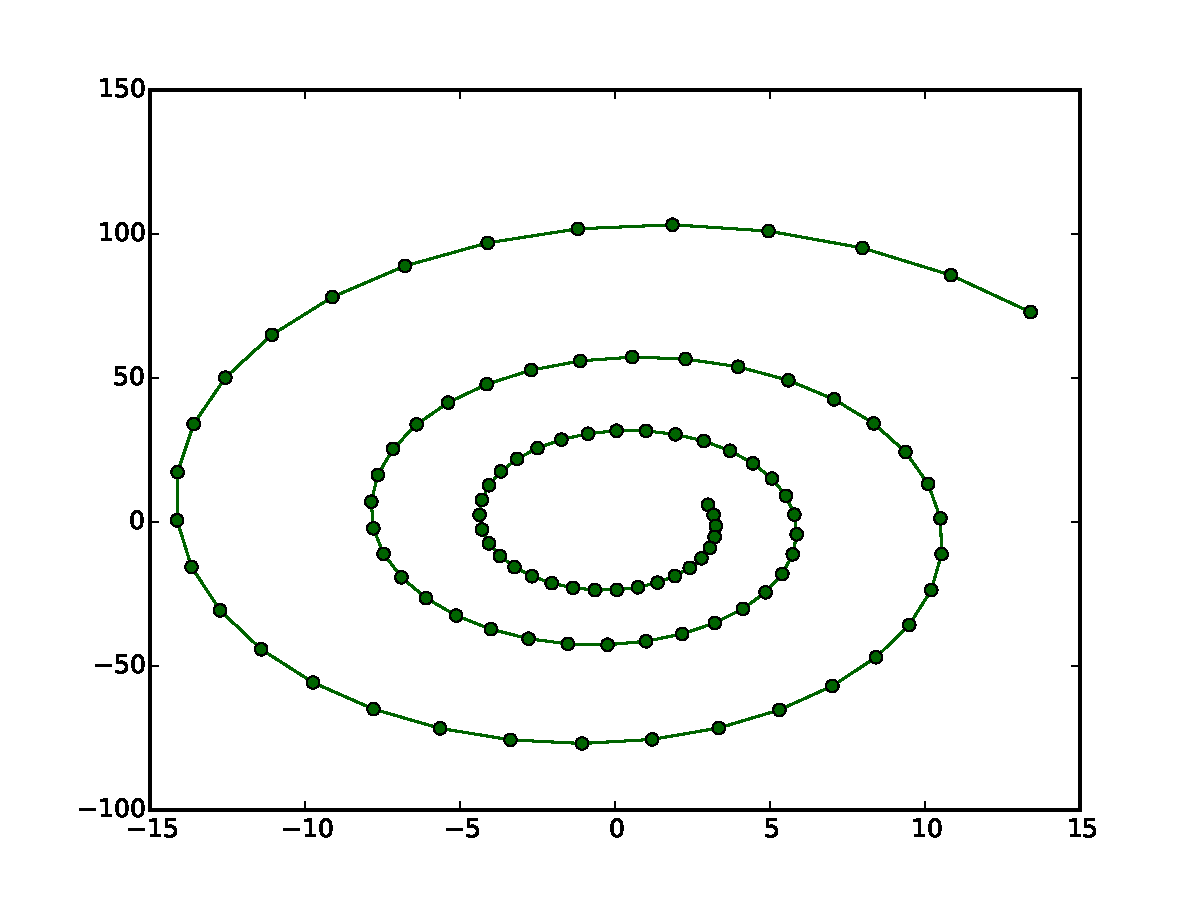
\includegraphics[width=9cm]{./Edyngrav_1_fig.pdf}
  % Edyngrav_1.pdf: 0x0 pixel, 300dpi, 0.00x0.00 cm, bb=
  \caption{Schéma d'Euler explicite}
  \label{fig:Edyngrav_1}
\end{figure}


\subsection*{II. \'Etude de schémas numériques}
Soit $y \in \mathcal{C}^2(\R)$ et $t_{min} < t_{max}$ deux réels. On note $I = \left[t_{min}, t_{max} \right]$. On s'intéresse à une équation différentielle du second ordre de la forme
\begin{equation}
  \forall t \in \R, \; y''(t) = f(y(t)) \label{eqdif}
\end{equation}
où $f$ est une fonction donnée continue sur $\R$.\newline
On suppose connues les valeurs $y_0=y(t_{min})$ et $z_0=y'(t_{min})$.
\begin{enumerate}
  \item On note $z=y'$.
\begin{enumerate}
  \item Vérifier que le système est \emph{conservatif} c'est à dire que, en notant $g$ une primitive de $f$, la fonction
\begin{displaymath}
  \forall t \in I, \; t \mapsto \frac{1}{2}y'(t)^2 - g(y(t))
\end{displaymath}
est constante. On note $E$ sa valeur. 
  \item Lorsque $y$ est solution de l'équation (\ref{eqdif}), exprimer $y'$ et $z'$ en fonction de $y$ et $z$. On note $(\mathcal{S})$ ce système obtenu.
  \item Soit $n$ un entier strictement supérieur à $1$ et $J_n = \llbracket 0, n-1\rrbracket$. On pose
\begin{displaymath}
  h = \frac{t_{max} - t_{min}}{n-1} \; \text{ et } \; \forall i\in J_n,\;t_i = t_{min} + i h
\end{displaymath}
Montrer que, 
\begin{equation}
  y(t_{i+1}) = y(t_i) + \int_{t_i}^{t_{i+1}}z(t)\, dt \;\text{ et } 
  z(t_{i+1}) = z(t_i) + \int_{t_i}^{t_{i+1}}f(y(t))\, dt \label{relint}
\end{equation}
\end{enumerate}
La suite du problème exploite les notations introduites dans cette partie et présente deux méthodes numériques dans lesquelles les intégrales précédentes sont remplacées par des valeurs approchées.

\item Schéma d'Euler explicite: chaque valeur de fonction sous le signe intégrale est remplacée par la valeur prise en la borne inférieure.
\begin{enumerate}
  \item Dans ce schéma, montrer que les relations \ref{relint} permettent de définir deux suites $\left(y_i \right)_{i\in J_n}$, $\left(z_i \right)_{i\in J_n}$ où $y_i$ et $z_i$ sont des valeurs approchées respectivement de $y(t_i)$ et $z(t_i)$. Donner les relations de récurrence permettant de déterminer les valeurs de $y_i$ et $z_i$ connaissant $y_0$ et $z_0$.
  \item \'Ecrire une fonction \texttt{euler} qui reçoit en argument les paramètres qui vous semblent pertinents et qui renvoie deux listes de nombres correspondant aux suites $\left(y_i \right)_{i\in J_n}$, $\left(z_i \right)_{i\in J_n}$. Vous justifierez le choix des paramètres transmis à la fonction.
\end{enumerate}

\item Pour illustrer cette méthode, on considère l'équation différentielle
\begin{displaymath}
  \forall t\in I,\; y''(t) = -\omega^2 y(t)
\end{displaymath}
dans laquelle $\omega$ est un nombre réel fixé.
\begin{enumerate}
  \item Montrer que $E=\frac{1}{2}\left( z(t)^2 + \omega^2 y(t)^2\right) $.
  \item Pour $i\in J_n$, on note $E_i$ la valeur approchée de $E$ à l'instant $t_i$ calculée en utilisant les valeurs approchées de $y(t_i)$ et $z(t_i)$ obtenues à la question 2.a. (schéma d'Euler explicite). Montrer que 
\begin{displaymath}
  E_{i+1} - E_i = h^2 \omega^2 E_i
\end{displaymath}
  \item En portant les valeurs de $y(t_i)$ sur l'axe des abscisses et les $z(t_i)$ sur celui des ordonnées, quelle serait l'allure de la courbe si l'énergie était conservée?
  \item Dans un système d'unité adapté,\label{misenoev} en prenant $y_0=3$, $z_0=6$, la mise en \oe{}uvre de la méthode d'Euler explicite génère la courbe de la figure \ref{fig:Edyngrav_1}. En quoi cette courbe confirme-t-elle que le schéma numérique ne conserve pas l'énergie? Justifier son allure et le sens dans lequel elle est parcourue.
\end{enumerate}

\item Schéma de Verlet. Il s'agit d'un schéma numérique d'intégration d'une équation de la forme \ref{eqdif} dans lequel, en notant $f_i=f(y_i)$ et $f_{i+1}=f(y_{i+1})$, les relations de récurrence s'écrivent
\begin{displaymath}
  y_{i+1} = y_{i} + hz_i + \frac{h^2}{2} f_i\hspace{0.5cm}\text{et}\hspace{0.5cm} z_{i+1} = z_i + h\,\frac{f_i + f_{i+1}}{2}
\end{displaymath}
La mise en \oe{}uvre de ce nouveau schéma dans les mêmes conditions que pour la question \ref{misenoev} conduit à la figure \ref{fig:Edyngrav_2}.
\begin{figure}[h]
  \centering
  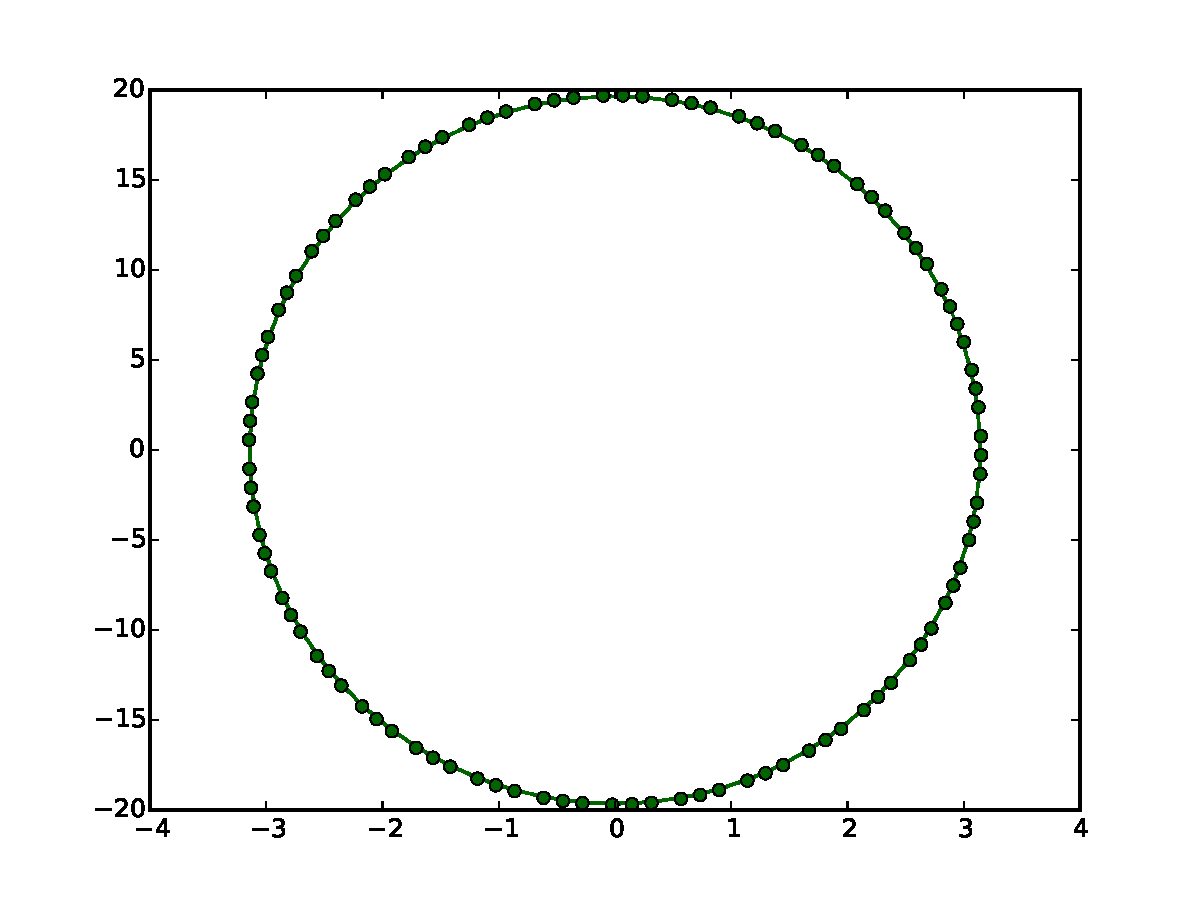
\includegraphics[width=9cm]{./Edyngrav_2_fig.pdf}
  % Edyngrav_1.pdf: 0x0 pixel, 300dpi, 0.00x0.00 cm, bb=
  \caption{Schéma de Verlet}
  \label{fig:Edyngrav_2}
\end{figure}
\begin{enumerate}
  \item \'Ecrire une fonction \texttt{verlet} qui reçoit en argument les paramètres qui vous semblent pertinents et qui renvoie deux listes de nombres correspondant aux suites $\left(y_i \right)_{i\in J_n}$, $\left(z_i \right)_{i\in J_n}$.
  \item \'Ecrire, pour le schéma de Verlet, des expressions de $y_{i+1}$ et $z_{i+1}$ puis $y_{i+1}^2$ et $z_{i+1}^2$ sous forme de développements limités en $O(h^3)$ ne contenant que $y_i$, $z_i$, $\omega$ et $h$.
  \item Formuler une conjecture expliquant les différences d'allure entre les courbes obtenues aux figures \ref{fig:Edyngrav_1} et \ref{fig:Edyngrav_2}. Prouver cette conjecture en utilisant les développements limités de la question précédente. 
\end{enumerate}
\end{enumerate}

\subsection*{III. Problème à $N$ corps.}
On s'intéresse à présent à la dynamique d'un système de $N$ corps massifs en interaction gravitationnelle ($N\geq 2$ entier naturel donné). Les corps considérés sont assimilés à des points matériels $P_j$ de masse $m_j$ avec $j\in \llbracket 0, N-1 \rrbracket$. Le mouvement de ces points est étudié dans un référentiel galiléen muni d'une base orthonormée. L'interaction entre deux corps $j$ et $k$ est modélisée par la force gravitationnelle. L'action exercée par le corps $k$ sur le corps $j$ est décrite par la force
\begin{displaymath}
  \overrightarrow{F}_{k\diagup j} = G\,\frac{m_j m_k}{r_{jk}^3}\, \overrightarrow{P_j P_k}\hspace{0.3cm} \text{avec} \hspace{0.3cm}
G=6.67\times 10^{-11}\,\text{N}.\text{m}^2.\text{kg}^{-2}  
\end{displaymath}
où $r_{jk} = \left\|\overrightarrow{P_j P_k}\right\|$ est la distance entre les corps $j$ et $k$ et $G$ est la constante de la gravitation universelle.\newline
\`A tout instant $t_i$ avec $i\in \llbracket 0,n \rrbracket$, l'état dynamique du corps $j$ est repéré par ses coordonnées cartésiennes $(x_{ij},y_{ij},z_{ij})$ et les coordonnées $(v_{xij},v_{yij},v_{zij})$ de son vecteur vitesse dans le référentiel fixé.\newline
Trois listes sont utilisées pour représenter ce système en Python.
\begin{itemize}
  \item \texttt{masse} conserve les masses de chaque corps: \texttt{masse[j]}$ = m_j$.
  \item \texttt{position} conserve les positions successives de chaque corps:\newline \texttt{position[i][j]} $=\left[ x_{ij}, y_{ij}, z_{ij}\right]$.
  \item \texttt{vitesse} conserve les vitesses successives de chaque corps:\\ \texttt{vitesse[i][j]} $=\left[ v_{xij}, v_{yij}, v_{zij}\right]$. 
\end{itemize}
L'objet de la fin de ce problème est de construire ces suites en mettant en \oe{}uvre le schéma de Verlet.
\begin{enumerate}
  \item Position du problème.
\begin{enumerate}
  \item Exprimer la force $\overrightarrow{F}_j$ exercée sur le corps $j$ par l'ensemble des autres corps.
  \item \'Ecrire une fonction \texttt{force2(m1,p1,m2,p2)} qui prend en paramètre les masses ($m1$ et $m2$ en kilogrammes) et les positions ($p1$ et $p2$ sous forme de listes de trois coordonnées cartésiennes en mètres) de deux corps 1 et 2 et qui renvoie la force exercée par le corps 2 sur le corps 1, sous la forme d'une liste à trois éléments représentant les coordonnées de la force dans la base de référence (en newtons).
  \item \'Ecrire une fonction \texttt{forceN(j,m,pos)} qui prend en paramètres l'indice $j$ d'un corps, la liste \texttt{m} des masses des $N$ corps, la liste \texttt{pos} des positions des $N$ corps et qui renvoie la force $\overrightarrow{F}_j$ exercée par tous les autres corps sur $j$ sous la forme d'une liste à trois éléments représentant les coordonnées de cette force dans la base du référentiel.
\end{enumerate}

\item Approche numérique.
\begin{enumerate}
  \item Expliciter la structure et la signification de \texttt{position[i]} et \texttt{vitesse[i]}.
  \item \'Ecrire une fonction \texttt{pos\textunderscore suiv(m, pos, vit, h)} qui prend en paramètres la liste de $N$ masses des corps (en kilogrammes), la liste de leurs positions (en mètres) à l'instant $t_i$, la liste de leurs vitesses (en mètres par secondes) au même instant, le pas d'intégration $h$ (en secondes) et qui renvoie la liste des positions des $N$ corps à l'instant $t_{i+1}$ calculés avec le schéma de Verlet.
  \item \'Ecrire une fonction \texttt{etat\textunderscore suiv(m, pos, vit,h)} qui prend les mêmes paramètres que la fonction \texttt{pos\textunderscore suiv} et qui renvoie la liste des positions (en mètres) et la liste des vitesses (en mètres par secondes) de $N$ corps à l'instant $t_{i+1}$ calculées en utilisant le schéma de Verlet. 
\end{enumerate}
  \item \'A titre de vérification, on expérimente numériquement dans le cas du problème des deux corps. Dans la page suivante\footnote{Pour ceux qui ne disposent que du noir et blanc: le petit tortillon et le petit ovale sont rouges.}, le code placé à gauche produit les images placées à droite. Commentez le code et les images. Les résultats obtenus vous semblent-ils cohérents?
\end{enumerate}
\newpage
\lstinputlisting[firstline=109, lastline=146]{Cdyngrav.py}
\begin{figure}[h]
  \centering
  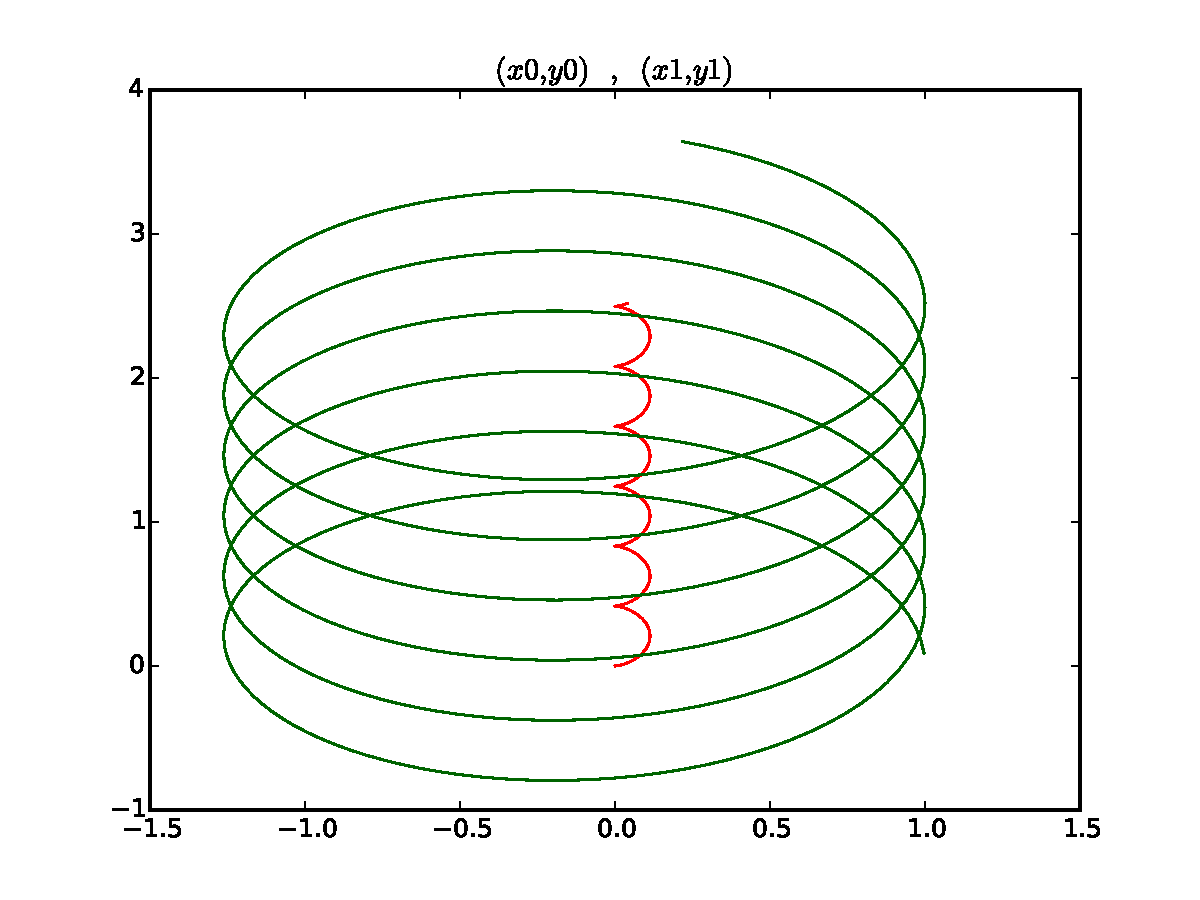
\includegraphics[width=10cm]{./Edyngrav_3_fig.pdf}
  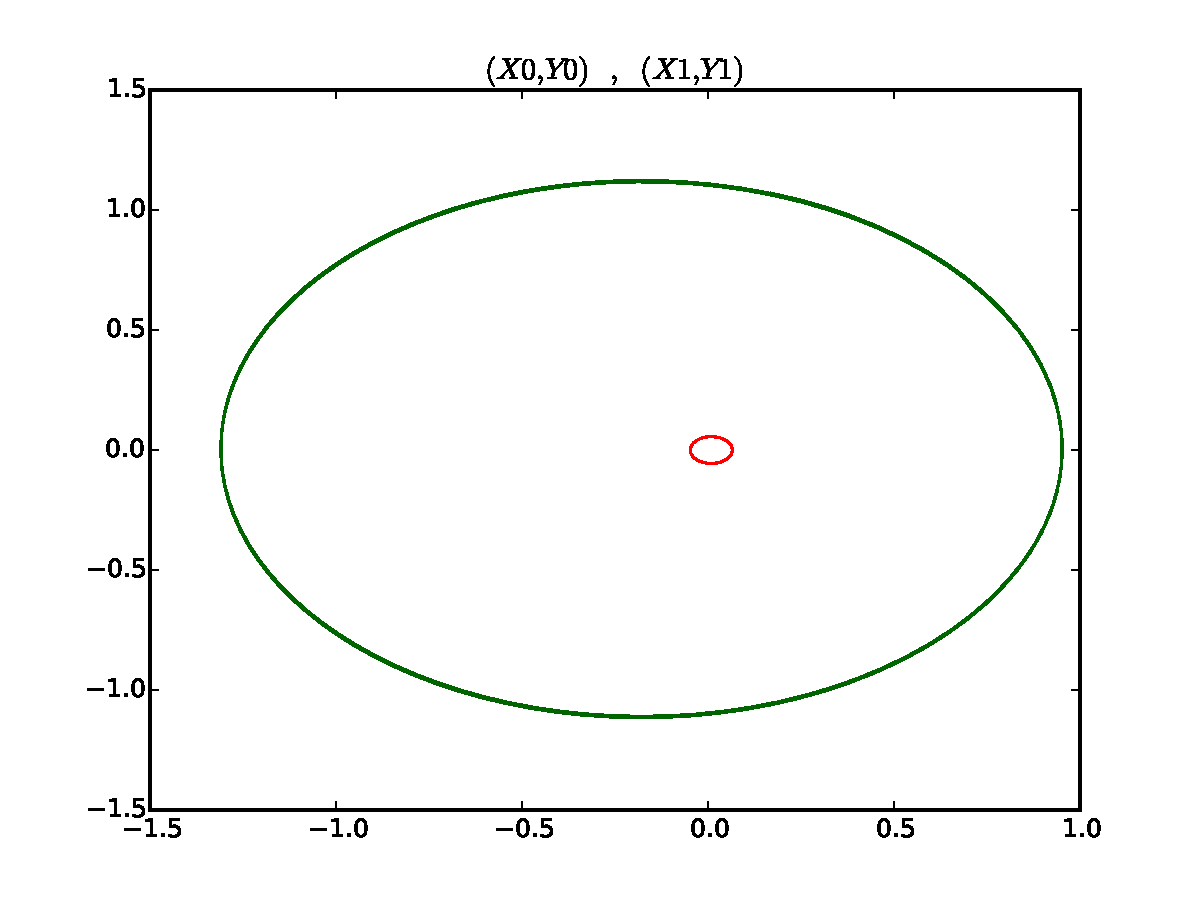
\includegraphics[width=10cm]{./Edyngrav_4_fig.pdf}
\end{figure}




